\chapter{Another Chapter}

\section{The first section}

Note that all section and chapter titles should use lower case except
for the first character of the first word. Here is a reference to a
paper~\cite{apaper}. Figure~\ref{fig:picture} is a weird picture.

\begin{figure}[h]
  \centering
  %% Because graphicspath was set in edengths.tex you only need to
  %% supply the file name here, i.e. examplepicture (doesn't need the
  %% extension) and not the full path. Just remember to add the path
  %% to \graphicspath{{thispath/}{thatpath/}}
  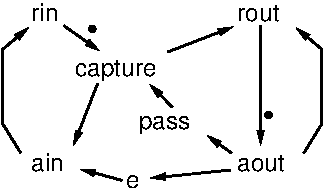
\includegraphics[width=2in]{examplepicture}
  \caption[Long caption and \textit{some italics} to see what happens]%
  {This is an example of pdf with a very long caption and \textit{some italics}
  to see what happens and it should see what happens over two lines.}
\label{fig:picture}
\end{figure}

\subsection{A subsection}

Lorem ipsum dolor sit amet, consectetur adipiscing elit. Maecenas nec orci 
lacus, ac sollicitudin tortor. Maecenas rutrum vestibulum rhoncus. Vestibulum 
non ligula nibh. Cum sociis natoque penatibus et magnis dis parturient montes, 
nascetur ridiculus mus. Phasellus egestas sodales lacus, ac scelerisque nulla 
venenatis sed. Ut elementum turpis ac lacus consectetur consequat. Sed at est 
eros. Praesent erat velit, dictum id adipiscing eu, ultrices vel nisi. Nullam 
at nisl ut est posuere commodo tincidunt eget nisl. Integer id erat non metus 
adipiscing dignissim quis sed enim. Curabitur viverra lobortis eleifend. Proin 
vestibulum nunc eu augue dapibus quis porttitor ipsum rhoncus. Duis tortor 
tellus, suscipit sit amet ornare id, lacinia sed lacus. Ut in molestie ligula. 
Praesent euismod lectus vitae arcu malesuada tempus. Aliquam pharetra 
tincidunt augue in eleifend. Curabitur porttitor vulputate quam, ut fringilla 
mauris porta eu. Curabitur sodales, felis non vestibulum feugiat, urna diam 
bibendum purus, ac scelerisque massa eros sit amet ipsum. In elementum laoreet 
aliquam.

\subsubsection{A subsubsection}

Aliquam eget sapien tellus, sed rutrum leo. Vestibulum et quam sit amet dolor 
gravida sagittis. Aenean dapibus urna a nibh sollicitudin pharetra. Sed nisi 
augue, vehicula sed tristique facilisis, lacinia ut augue. Nam quis tempor mi. 
Vestibulum lorem leo, aliquet at sollicitudin vitae, fringilla id odio. Aenean 
a orci odio. Mauris tincidunt eros ac libero suscipit molestie. Donec feugiat 
turpis a urna suscipit in pellentesque magna pretium. Vivamus eget nunc vitae 
nunc ultricies tincidunt. Duis dictum eros et lorem auctor id ullamcorper diam 
commodo. Pellentesque quis dolor nec urna vestibulum pellentesque. Donec 
luctus mi ut nisi hendrerit pulvinar. Donec fringilla, lectus vitae accumsan 
sollicitudin, sem metus mollis risus, nec laoreet ante arcu ut augue.

\subsection{Another subsection}

Table~\ref{tab:atable} is an example of a~\footnote{this is a
footnote} simple table.

\begin{table}[htb]
\begin{center}
\begin{tabular}{|c|c|c|}
\hline
1.0 & 2.0 & 3.0 \\
\hline
4.0 & 5.0 & 6.0 \\
\hline
\end{tabular}
\caption{A table}
\label{tab:atable}
\end{center}
\end{table}


\section{Another section}

This is a long and boring paragraph for the purpose of testing the
spacing between paragraphs and the use or otherwise of indentation. I
think a space between paragraphs and without the first line indented
is somewhat easier to read than no space between paragraphs and with
the first line indented.

Another equally exciting paragraph, one two three four five six seven
eight nine ten eleven twelve thirteen fourteen fifteen sixteen
seventeen eighteen nineteen twenty and so on.

\begin{equation} \label{eqn:dct}
z(k,l) = \frac{2}{N} \alpha(k) \alpha(l) \sum_{m=0}^{N-1} \sum_{n=0}^{N-1}
         x(m,n) \cos \frac{ (2m+1) \pi k}{2N} \cos \frac{ (2n+1) \pi l}{2N}
\end{equation}

\begin{equation} \label{eqn:idct}
x(m,n) = \frac{2}{N} \sum_{k=0}^{N-1} \sum_{l=0}^{N-1}
         \alpha(k) \alpha(l) z(k,l)
\end{equation}

\begin{quotation}
This is a quotation, another equally exciting paragraph, one two three
four five six seven eight nine ten eleven twelve thirteen fourteen
fifteen sixteen seventeen eighteen nineteen twenty and so on. Just
checking it is single spaced.
\end{quotation}

\section{Section with a landscape image}

\Autoref{fig:landscape} is an image on a landscape orientated page with
the header removed and a simple footer added.

\begin{landscape}
\thispagestyle{plain} % Remove this line for normal headers
\begin{figure}[p]
  \centering
    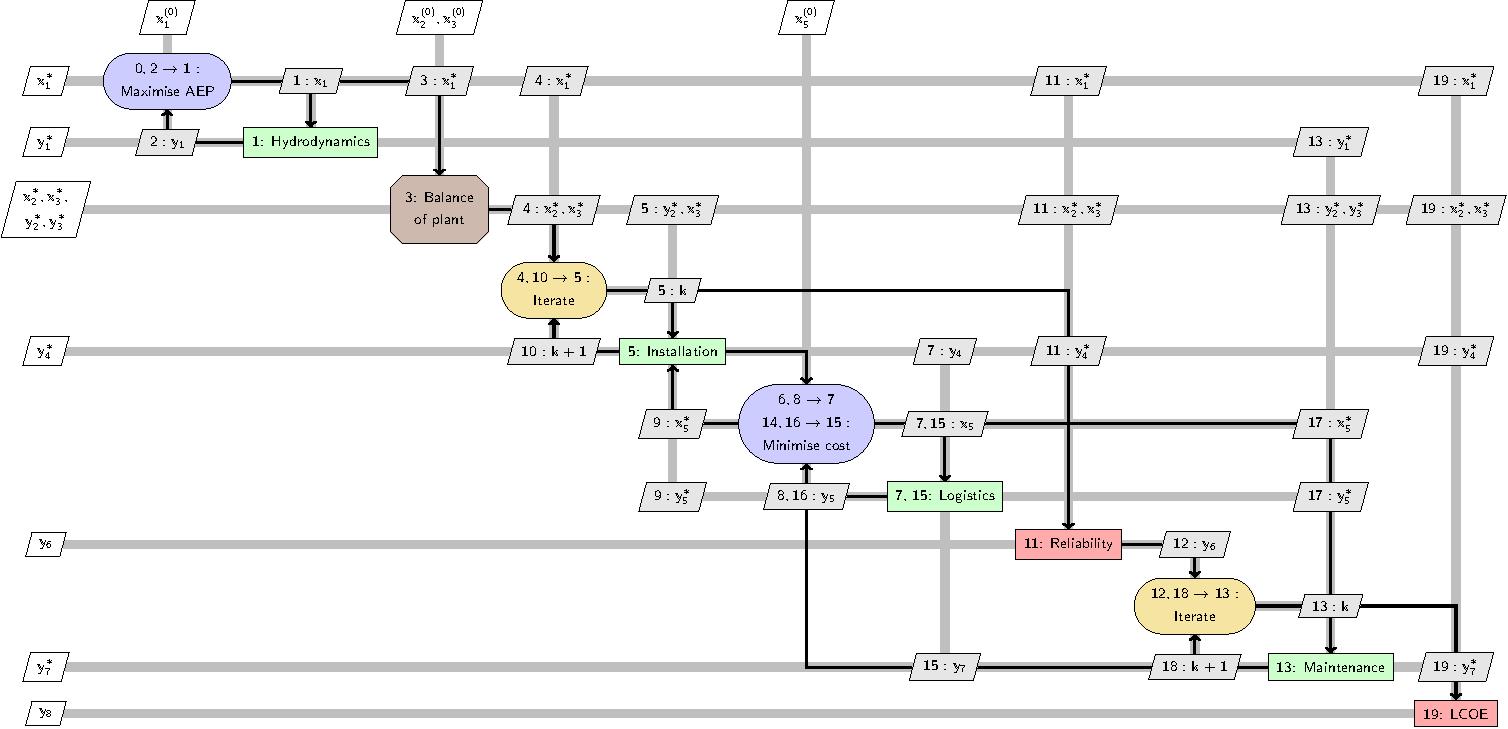
\includegraphics[width=\linewidth]{xdsm_sequential-crop}
    \caption{XDSM diagram. Reproduced from \citep{topper2021}.
    \label{fig:landscape}
}
\end{figure}
\end{landscape}
